\documentclass{article}
\usepackage{graphicx,dcolumn,bm,verbatim,hyperref,color,tabularx,enumitem,soul,floatrow,caption,layout,amsmath,amssymb,mathtools,quantikz,wrapfig,lipsum,tikz} % Required for inserting images
\usetikzlibrary{patterns}
\usepackage[sorting=none]{biblatex}
\addbibresource{export.bib}
\setlength{\hoffset}{10pt}
\setlength{\voffset}{-40pt}
\setlength{\headsep}{0pt}
\setlength{\oddsidemargin}{0pt}
\setlength{\textwidth}{450pt}
\setlength{\textheight}{660pt}
\title{Basic theory of a standing wave optical cavity in vacuum}

\date{February 2026}

\author{Alexei Gurchenko}


\begin{document}

\maketitle

\section{Reflected, transmitted and intracavity fields}

Let us start by calculating the reflected, transmitted and intracavity fields. Figure \ref{fig:cavity} depicts the schematic of the electromagnetic wave traveling inside the optical cavity. We assume that the mirrors $1$ and $2$ have corresponding amplitude transmission and reflection coefficients $r_1$, $t_1$ and $r_2$, $t_2$. The intracavity medium is lossless, however there is a loss of amplitude due to scattering at the mirror surfaces: $t_a$ at Mirror $1$ and $t_b$ at Mirror $2$. This model is the closest approximation of a two-mirror cavity inside ultra-high vacuum environment.


\begin{figure}[H]
    \centering
    \begin{tikzpicture}[x=1cm,y=1cm,>=Latex, line cap=round, line join=round]

        % --- geometry parameters
        \def\xL{0}        % mirror 1 x
        \def\xR{12}       % mirror 2 x

        \def\yTop{1.3}
        \def\yMid{0.5}
        \def\yBot{-0.3}
        \def\yBotB{-1.1}

        \def\boxL{4.5}
        \def\boxR{9.5}
        \def\boxB{-1.6}
        \def\boxT{2.0}
        \def\arrmarg{1.0}

        % --- mirrors (hatched)
        \draw[pattern=north east lines] (\xL-0.18,\boxB-0.2) rectangle (\xL+0.08,\boxT+0.2);
        \draw[pattern=north east lines] (\xR-0.08,\boxB-0.2) rectangle (\xR+0.18,\boxT+0.2);
        \filldraw (\xL+0.08,\boxB-0.2) rectangle (\xL+0.18,\boxT+0.2);
        \filldraw (\xR-0.08,\boxB-0.2) rectangle (\xR-0.18,\boxT+0.2);

        \node[below] at (\xL,\boxB-0.25) {Mirror 1};
        \node[below] at (\xR,\boxB-0.25) {Mirror 2};

        % --- labels above mirrors
        \node[above] at (\xL, \boxT+0.35) {$t_1\ \ r_1\ \ t_a$};
        \node[above] at (\xR, \boxT+0.35) {$r_2\ \ t_2\ \ t_b$};

        % % --- lossy medium box
        % \draw (\boxL,\boxB) rectangle (\boxR,\boxT);
        % \node at ({(\boxL+\boxR)/2},{(\boxB+\boxT)/2}) {Lossy medium};
        % \node at ({(\boxL+\boxR)/2},{\boxT-0.55}) {$t$};


        % arrows
        \draw[-Latex,thick] (-2,\yTop) -- (\xL-0.18,\yTop); %input
        \draw[-Latex,thick] (\xL+0.18,\yTop) -- (\xR-0.18,\yTop); %first
        \draw[-Latex,thick] (\xR+0.18,\yTop) -- (\xR+1.4,\yTop); % first transmission
        \draw[-Latex,thick] (\xR-\arrmarg,\yMid) -- (\xL+0.18,\yMid); %second 
        \draw[-Latex,thick] (\xL-0.18,\yMid) -- (\xL+-1.4,\yMid); %second reflection
        \draw[-Latex,thick] (\xL+\arrmarg,\yBot) -- (\xR-0.18,\yBot); %third
        \draw[-Latex,thick] (\xR+0.18,\yBot) -- (\xR+1.4,\yBot); %third transmission
        \draw[-Latex,thick] (\xR-\arrmarg,\yBotB) -- (\xL+0.18,\yBotB); %fourth
        \draw[-Latex,thick] (\xL-0.18,\yBotB) -- (\xL-1.4,\yBotB); %fourth reflection



        % reflection loops
        \draw[thick] (\xR-\arrmarg,\yTop) .. controls (\xR,\yTop) and (\xR,\yMid) .. (\xR-\arrmarg,\yMid); %1-2
        \draw[thick] (\xL+\arrmarg,\yMid) .. controls (\xL,\yMid) and (\xL,\yBot) .. (\xL+\arrmarg,\yBot); %2-3
        \draw[thick] (\xR-\arrmarg,\yBot) .. controls (\xR,\yBot) and (\xR,\yBotB) .. (\xR-\arrmarg,\yBotB); %3-4
        \draw[-Latex,thick] (\xL-\arrmarg,\yTop) .. controls (\xL,\yTop) and (\xL,\yTop+0.8) .. (\xL-\arrmarg,\yTop+0.8); %0

        % another round-trip sketch (one more loop at mirror 2 and back) to suggest series




        % --- distance L arrow
        \draw[Latex-Latex] (\xL,\boxB-1) -- (\xR,\boxB-1);
        \node[below] at ({(\xL+\xR)/2},\boxB-0.5) {$L$};

    \end{tikzpicture}
    \caption{Optical cavity schematic}
    \label{fig:cavity}
\end{figure}

\subsection{Reflection and transmission at an interface}

The first question we need to answer before moving on to calculating reflected field, is the following. If light is shined to an interface from one side and the interface has reflected coefficient $r$ and transmitted coefficient $t$, what would be the reflected and transmitted coefficients $r'$ and $t'$ if the light is shined from another side? This elegant derivation \cite{Nagourney2014} of the relation between the field transmission and reflection
coefficients was made by the British physicist Sir George Gabriel Stokes. He assumed that there was no dissipation at the interface and therefore the process obeyed time-reversal invariance. The three waves are shown on the left in the figure. The time-reversed case appears in the center plot. When we reverse time, we need to include three additional waves: the reflection from the bottom wave, and the transmission of both the bottom and top waves. All of the waves are shown in the plot on the right. In order for the right-hand plot to be equivalent to the time-reversed center plot, the two waves in the upper left must sum to E and the two waves in the lower left must
sum to zero. Thus, $$E = E t t' + E r r' \text{  and  } 0 = E r t + E r' t $$




\printbibliography

\end{document}
